\section{Bifurkationen}
\exercise{Grundlagen}
Beantworte die folgenden Fragen
\begin{itemize}
    \item Was ist eine Bifurkation?
    \item Wann entsteht eine Bifurkation?
    \item Was ist das mathematische Kriterium für eine Bifurkation?
    \item Welche Formen von Bifurkationen gibt es?
    \item Was können Beispiele für Biologische Systeme mit Bifurkationen sein? (2 Stück)
\end{itemize}
%
%
\exercise{Python erstes Beispiel}
Das python-script "Bifurkationen.py" bietet eine erste einfache Möglichkeit, Bifurkationen zu plotten.
Es ist noch leicht unvollständig.
Verstehe das Skript und vervollständige es.
Das Endergebnis sollte dann aussehen wie in Figur~\ref{fig:bifurcation-plot}.
\begin{figure}[!h]
    \centering
    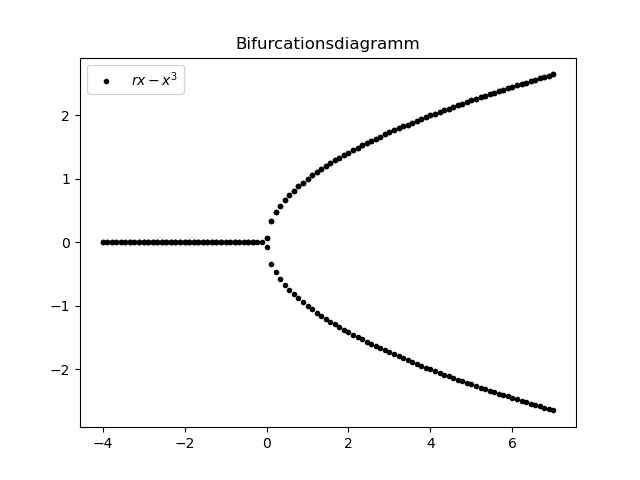
\includegraphics[width=0.6\textwidth]{media/Bifurkationsplot.png}
    \caption{Bifurkation geplottet mit python}
    \label{fig:bifurcation-plot}
\end{figure}
%
%
\exercise{Auf Papier: Erwartungen an Systeme}
Betrachte die folgenden Gleichungen jeweils als einzelstehende \acp{ode}. Welche davon zeigen Bifurkationen? Welche weiteren Verhaltensweisen sind zu erwarten? Wie viele Gleichgewichtszustände gibt es?
\begin{align}
    \dot{x} &= -rx^3+x\\
    \dot{x} &= x - rx^3\\
    \dot{x} &= ax + bx^2 - rx^3\\
    \dot{x} &= -(x-r)(x-1+r)^2 - (x-r)^2(x-1+r)\\
    \dot{x} &= -\frac{\partial}{\partial x}\left(1-\e(-(x-r)^2)\right)^2\left(1-\e(-(x-1+r)^2)\right)^2\\
    \dot{x} &= -\frac{\partial V}{\partial x}(x)
\end{align}
wobei $g(x)$ gegeben ist durch Diagramme aus Figur~\ref{fig:potential-plots}.
\begin{figure}[!h]
    \centering
    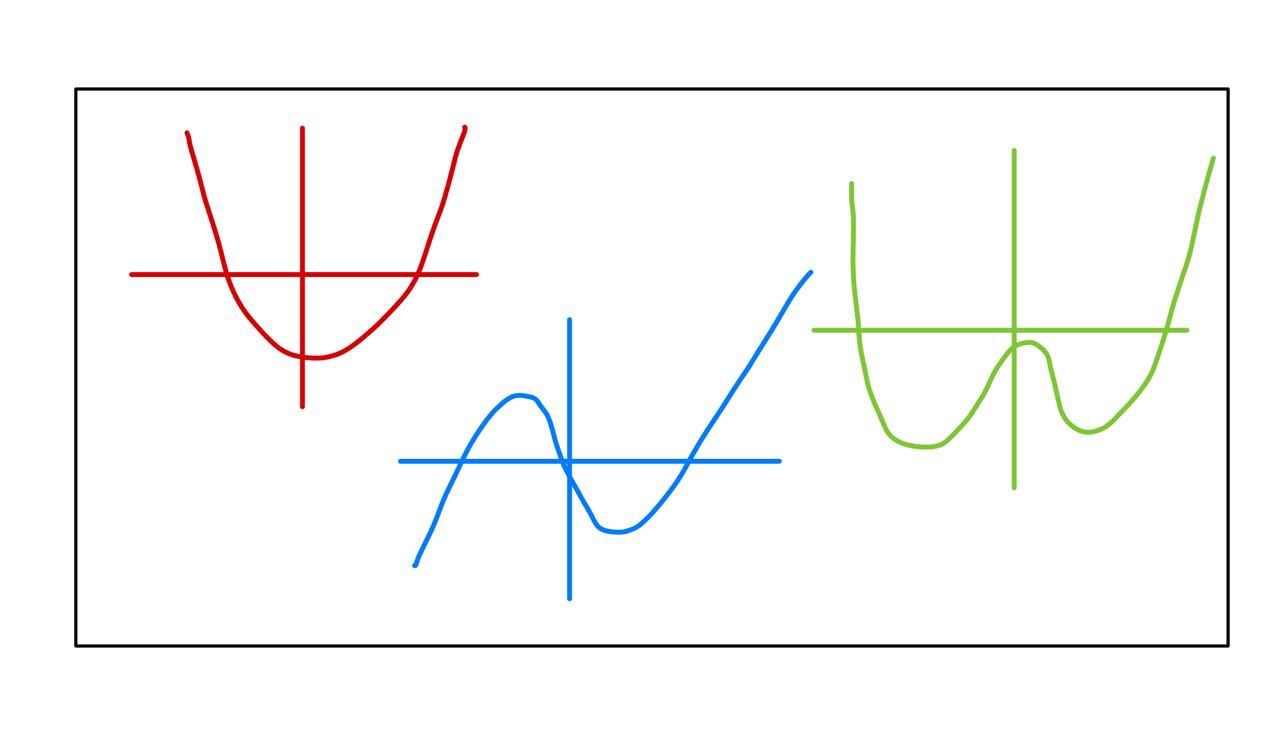
\includegraphics[width=0.75\textwidth]{media/potential-plots.jpg}
    \caption{Plots für Möglichkeiten von $V(x)$.}
    \label{fig:potential-plots}
\end{figure}
%
%
\exercise{Erwartungen überprüfen}
Benutze das python-script von zuvor, um die oben beschriebenen Systeme zu plotten und mit deinen Erwartungen zu vergleichen.
%
%
\exercise{Hopf-Bifurkation (Zusatz)}
Wie müsste man das vorheregangene Muster verändern, um eine Hopf-Bifurkation zu visualisieren?
Schreibe ein Python-script für die folgende \ac{ode}
\begin{align}
    \dot{x} &= \lambda(x+y) + \alpha(x^2+y^2)\\
    \dot{y} &= x+y+\beta(x^2+y^2)
\end{align}
Für welche Werte von $\lambda,\alpha,\beta$ finden wir Bifurkationen, stabile Fixpunkte etc.?
%
%
\section{Toggle-Switch Model}
%
%
\exercise{Grundlagen}
Beantworte die folgenden Fragen
\begin{itemize}
    \item Gehört dieses System von \acp{ode} zu einer Reaktion, die wir aufschreiben können?
    \item Was möchte man mit diesem mathematischen model biologisch simulieren?
    \item Was ist eine Nullcline? Warum ist sie hilfreich?
\end{itemize}
%
%
\exercise{Analyse des Models}
...
%
%